\documentclass[11pt,aspectratio=169,svgnames]{beamer}

\usefonttheme{professionalfonts}

\usepackage{amsmath,amssymb,amsthm,mathtools}
\usepackage{xcolor,graphicx,tikz}
\usepackage[russian]{babel}

\definecolor{dgray}{RGB}{15,15,15}
\definecolor{dplot}{HTML}{96e6ff}

\usebackgroundtemplate{%
	
\includegraphics[width=\paperwidth,height=\paperheight]{img/lile-back-dgray}%
}

\setbeamersize{text margin left=12mm,text margin right=12mm}
\addtolength{\headsep}{0.55cm}
\setbeamertemplate{frametitle}[default][left,leftskip=0.85cm]
\setbeamertemplate{navigation symbols}{}
\setbeamertemplate{blocks}[rounded]
\setbeamertemplate{footline}{\vspace{1.4cm}}

\setbeamercolor{titlelike}{fg=white}
\setbeamercolor{normal text}{fg=white}
\setbeamercolor{block title}{bg=white!27!dgray,fg=white}
\setbeamercolor{block body}{bg=white!10!dgray}

\DeclarePairedDelimiter{\lr}{(}{)}
\DeclarePairedDelimiter{\atdeg}{[}{]}
\newcommand{\br}{\mathbb{R}}

\usepackage{mathspec}

\setsansfont[
	Path = f/,
	Extension = .otf,
	BoldFont=fb,
	BoldItalicFont=fbi
		]{f}
		
\setmathfont(Digits)[Path = f/]{roboto.ttf}
\setmathfont(Latin)[Path = f/]{robotoi.ttf}
\setmathfont(Greek)[Path = f/, Uppercase]{roboto.ttf}
\setmathfont(Greek)[Path = f/, Lowercase]{robotoi.ttf}


\newenvironment{nblock}[1]{
	\begin{center} \begin{columns}[t] \begin{column}{110mm} \begin{block}{#1}
   }{
	\end{block} \end{column} \end{columns} \end{center}
}

\newcommand{\graslide}[2]{
   \begin{frame} \frametitle{#1}
      \includegraphics[width=0.88\textwidth]{python-convolution/#2}
   \end{frame}
}

\newcommand{\probtitle}{Распределение сред. арифметического, \(f * \ldots * f\)}

   \title{О свёртке и её применениях}
   \date{\today}
   \author{Золотов Борис Алексеевич, аспирант МКН СПбГУ, \\ преподаватель ЛНМО}
   \institute{«Лига Лекторов», 3 сезон}

\begin{document} \maketitle

\section{Пример: умножение многочленов}

\begin{frame} \frametitle{Умножение многочленов}
	\[\lr*{3x^3 + 5x^2 + 2x + 7} \cdot \lr*{x^3 + 6x^2 + 8x + 4}\]

	Как формируется коэффициент при данной степени? \medskip \\ \pause
	Например, при \(x^4\):
	\[3 \cdot 8 + 5 \cdot 6 + 2 \cdot 1.\] \pause

	Иными словами, мы можем сказать, что
	\[A \cdot B\atdeg*{x^n} =
	  \sum\limits_{k+\ell=n} A\atdeg*{x^k} \cdot B\atdeg*{x^\ell}.\]
\end{frame}

\section{Пример: ковид}

\graslide{График заболеваемости ковидом}{covid-0}
\graslide{График заболеваемости ковидом}{covid-1}
\graslide{Недельное среднее:\quad \(\sum \lr*{\frac17 \cdot S(d)}\)}{covid-2}

\section{Пример: сумма чисел на двух кубиках}

\begin{frame} \frametitle{Сумма чисел на двух кубиках}

\begin{center} \tikz[scale=0.7]{
   \foreach \s in {1,...,6} {
	\filldraw[fill=dplot,fill opacity=0.15,rounded corners=1.2mm]
	   (1.45 * \s, 0) rectangle ++ (1,1);
	\filldraw[fill=dplot,fill opacity=0.15,rounded corners=1.2mm]
	   (1.45 * \s, -1.8) rectangle ++ (1,1);
	\node at (1.45 * \s + 0.5, 0.5)		{\s};
	\node at (10.65 - 1.45 * \s, -1.3)	{\s};
   }
} \end{center}

С какой вероятностью сумма выпавших чисел равна 5? \pause
	\[ 4 \cdot \lr*{\frac16}^2.\] \pause

Иными словами,
	\[ P_Σ \lr*{n} = \sum\limits_{k+\ell=n} P_1 \lr*{k} \cdot P_2 \lr*{\ell}. \]

\end{frame}

\section{Определение свёртки}

\begin{frame} \frametitle{Общее определение свёртки}
Пусть \(\lr*{S, \circ}\)~— множество с какой-то операцией (сложение, \\
умножение, взятие максимума\ldots). \\
Пусть \(f, g \colon\; S \to \br\), тогда
	\[ f * g \colon\; S \to \br,\quad
	   f * g \lr*{x} = \sum_{p\:\circ_S\: q = x} f(p)\:\cdot_\br\: g(q). \] \pause

Если \(S = \br\), то сумма превращается в интеграл:
	\[ f * g \lr*{x} = \int\limits_\br f(t) \cdot g(x-t) \cdot dt.\]
\end{frame}

\section{Применение: операции с изображениями}

\begin{frame} \frametitle{Блюр — это свёртка (\(\circ\) — покоординатное сложение)}
	\begin{center}
	   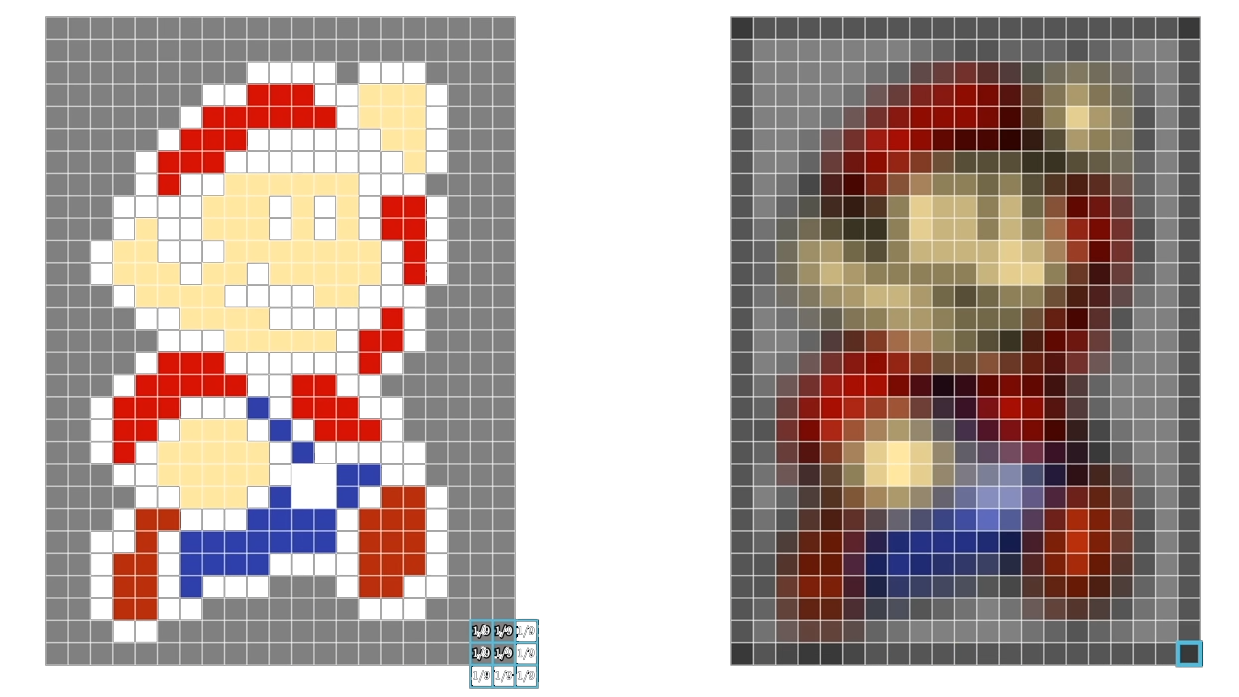
\includegraphics[width=0.75\textwidth]{img/conv-blur}
	\end{center}
\end{frame}

\begin{frame} \frametitle{Среднее с весами: гауссовский блюр}
	\begin{center}
	   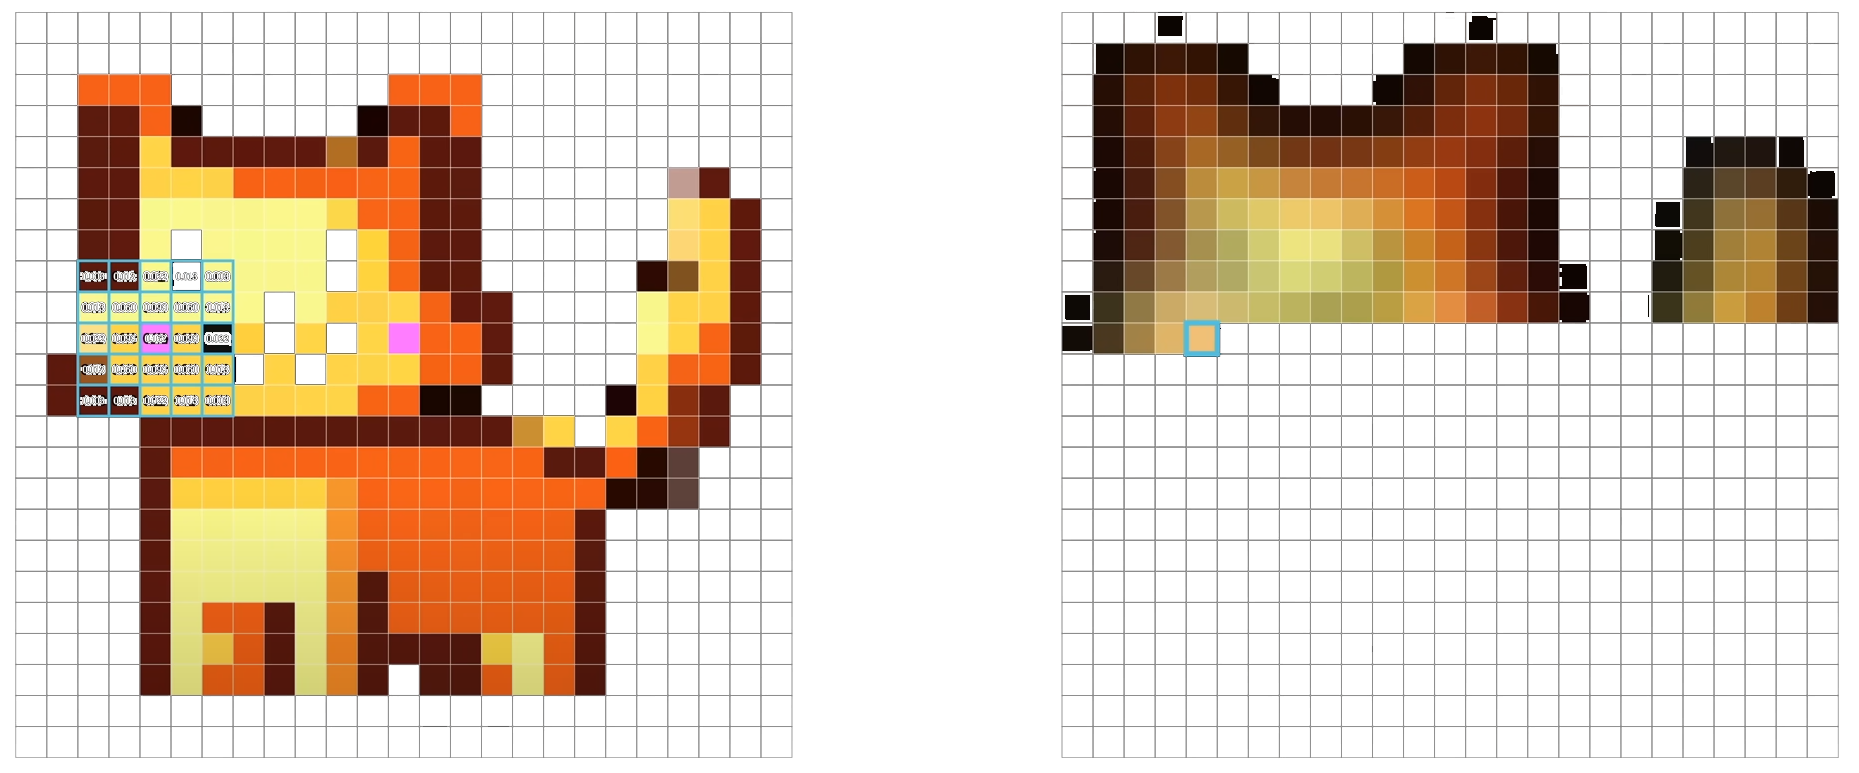
\includegraphics[width=0.75\textwidth]{img/conv-gaussian}
	\end{center}
\end{frame}

\begin{frame} \frametitle{Определение краёв и другие операции}
	\begin{center}
	   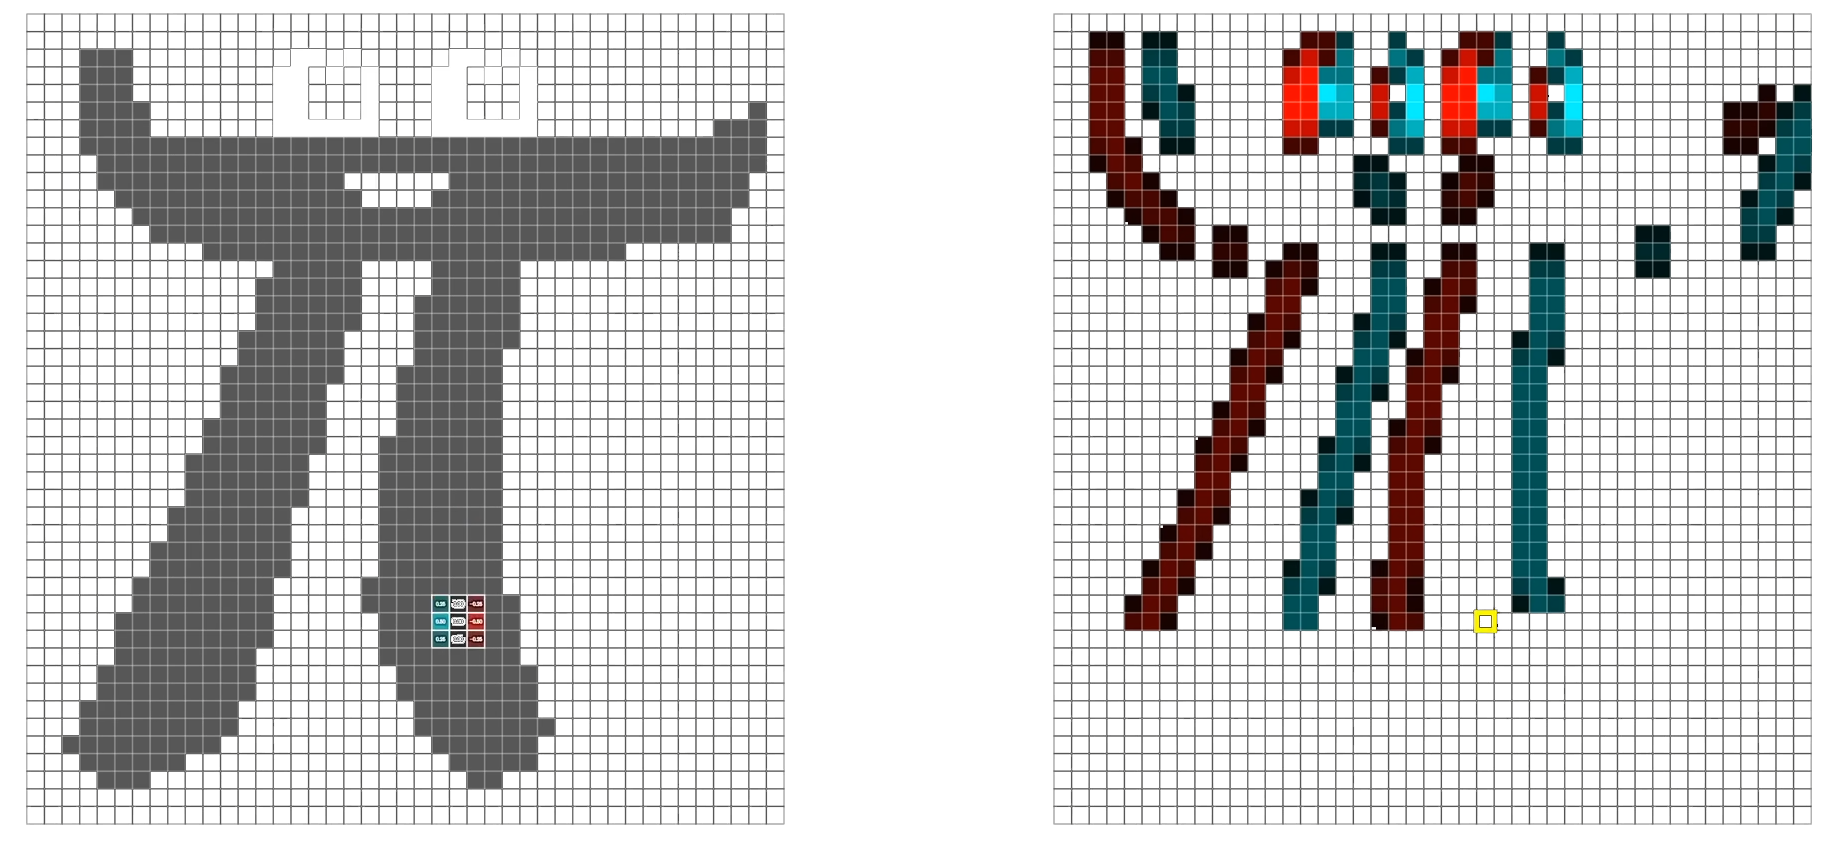
\includegraphics[width=0.75\textwidth]{img/conv-ridge}
	\end{center}
\end{frame}

\section{Применение: сглаживание функций (и уравнение теплопроводности)}

\begin{frame} \frametitle{Приближение гладкими функциями}
	Дана функция \(f\)~— совершенно точно не гладкая,\\
	но взятая из практики. \bigskip \\

	Хочется приблизить её гладкими (чтобы интегрировать, \\
	искать максимум, etc.). \bigskip \\

	Идея: взять скользящее среднее, но, желательно, \\
	«уважающее» значение в данной точке.	
\end{frame}

\graslide{Нормальное распределение}{normal}
\graslide{Рассмотрим негладкую функцию}{smoothing-0}
\graslide{Приблизим гладкими: \(f * \text{гаусс}\)}{smoothing-2.00}
\graslide{Приблизим гладкими: \(f * \text{гаусс}\)}{smoothing-1.00}
\graslide{Приблизим гладкими: \(f * \text{гаусс}\)}{smoothing-0.50}
\graslide{Приблизим гладкими: \(f * \text{гаусс}\)}{smoothing-0.20}
\graslide{Приблизим гладкими: \(f * \text{гаусс}\)}{smoothing-0.05}

\begin{frame} \frametitle{Уравнение теплопроводности}
	Оказывается, свёртка с гауссовой функцией — это \\
	решение уравнения теплопроводности: как будет \\
	распределяться температура по неравномерно \\
	нагретому стержню.
\end{frame}

\section{Ещё применения и конец презентации}

\begin{frame} \frametitle{Ещё применения}
	Зачем вообще обзывать много действий из жизни \\
	одной абстрактной операцией? Чтобы сразу для всех \\
	доказывать свойства и искать \\
	способы быстро вычислять (FFT). \bigskip

\begin{itemize}
	\item Умножение матриц и его ассоциативность
	\item Арифметическая свёртка: \(μ * I = \text{id}\), потом вылезет в \(ζ\) Римана
	\item Степенные ряды: обратимость и линейные рекурренты
	\item Центральная предельная теорема — это про \(f * f * \ldots\)
\end{itemize}
\end{frame}

\graslide{\probtitle}{probability-0}
\graslide{\probtitle}{probability-1}
\graslide{\probtitle}{probability-2}
\graslide{\probtitle}{probability-3}
\graslide{\probtitle}{probability-4}
\graslide{\probtitle}{probability-5}

\end{document}

\begin{frame} \frametitle{}
\end{frame}

\begin{nblock}{\vspace*{-3ex}}
	Sample text
\end{nblock}
